\documentclass[../../index.tex]{subfiles}

\begin{document}
\chapter{Introduction}
In particle physics we are concerned about small objects and their interactions.
The smallest of these objects are referred to as \textit{elemental particles}.
Their dynamics are governed by the laws of nature. These laws are organised
through symmetries, which are currently best described by the
\define{sm}{Standard Model}.

The \textsc{sm} classifies all known elementary particles and describes three of
the four fundamental forces: the electromagnetic, weak and strong force. The
particles representing matter are contained in two groups of fermionic,
spin\-/1/2 particles. The former group, the leptons consist of: the electron
(\(e\)), the muon (\(\mu\)), the tau (\(\tau\)) and their corresponding
neutrinos \(\nu_e\), \(\nu_\mu\) and \(\nu_\tau\). The latter group, the quarks
contain: \(u\), \(d\) (up and down, the so called light quarks ), \(s\)
(strange), \(c\) (charm), \(b\) (bottom or beauty) and \(t\) (top or truth). The
three fundamental forces, the \textsc{sm} differentiates, are described through
their carrier particles, the so\-/called bosons: the photon for the
electromagnetic, the \(Z\) or \(W\) boson for the weak and the gluon (\(g\)) for
the strong interaction. The before mentioned Leptons solely interact through the
electromagnetic and the weak force (also referred to as electroweak
interaction), whereas the quarks additionally interact through the strong force.
A short summary of the taxonomy of the \textsc{sm} can be seen in
\cref{fig:SMTaxonomy}
\begin{figure}
  \centering
  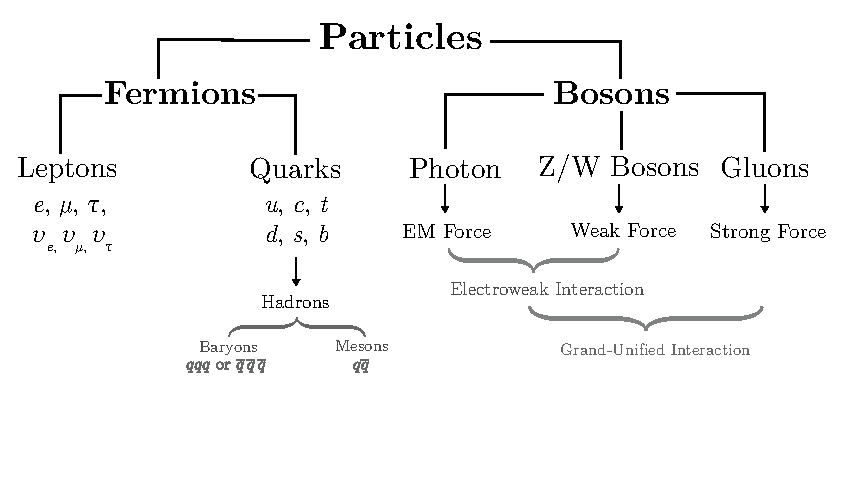
\includegraphics[width=\textwidth]{./images/standardModelTaxonomy.eps}
  \caption{Taxonomy of the Standard Model.}
  \label{fig:SMTaxonomy}
\end{figure}

From a more mathematical point of view the \textsc{sm} is a gauge
\define{qft}{quantum field theory}, which is a combination of \textit{classical
  field theory}, \textit{special relativity} and \textit{quantum mechanics}. Its
fundamental objects are ruled through its gauge\-/group \(SU(3)\times
SU(2)\times U(1)\). Each of its subgroups introduces a global and a local gauge
symmetry. The global symmetry introduces the charges, which the fields are
carrying. The local symmetry introduce the gauge-fields, which represent the
previously mentioned force carriers. Naively every subgroup\footnote{Actually
  \(U(1)\) and \(SU(2)\) have to be regarded as combined group to be mapped to
  the electromagnetic\-/ and weak\-/force in form of the electroweak
  interaction.} of the gauge\-/group of the standard model is responsible for
one of the three forces:
\begin{description}
\item[\(\bm{U(1)}\)] the \textit{abelian} gauge group governs the representation
  of \textit{quantum electrodynamics} (\textsc{qed}), which is commonly known as
  the electric force. Its global and local symmetry introduces the electric
  charge and the photon\-/field.
\item[\(\bm{SU(2)}\)] Is the \textit{non\-/abelian} symmetry group responsible
  for the weak\-/interaction. It introduces the \(W^+,W^-\) and \(Z\) bosons and
  the weak charge. The gauge groups \(U(1)\) and \(SU(2)\) have been combined to
  the \textit{electroweak interaction}.
\item[\(\bm{SU(3)}\)] The \(SU(3)\)\-/group is also \textit{non-abelian} and
  governs the strong interactions, which are summarised in the theory of
  \define{qcd}{Quantum Chromodynamics}. The group yields the three colour
  charges and due to its eight\-/dimensional adjoint\-/representation, eight
  different gluons.
\end{description}
Unfortunately we are still not able to include gravity, the last of the four
forces, into the \textsc{sm}. There have been attempts to describe gravity
through \textsc{qft} with the graviton, a spin\-/2 boson, as mediator, but there
are unsolved problems with the renormalisation of general relativity
(\textsc{gr}). Until now \textsc{gr} and quantum mechanics (\textsc{qm}) remain
incompatible.

Apart from gravity not being included, the \textsc{sm} has a variety of flaws.
One of them is being dependent on many parameters, which have to be measured
accurately to perform high\-/precision physics. In total the Lagrangian of the
\textsc{sm} contains 19 parameters. These parameters are represented by ten
masses, four \textsc{ckm}\-/matrix parameters, the \textsc{qcd}\-/vacuum angle,
the Higgs\-/vacuum expectation value and three gauge coupling constants. Highly
accurate values with low errors are crucial for theoretical calculated
predictions. One of the major error inputs of every theoretical output are
uncertainties in these parameters. In this work we will focus on one of the
parameters, namely the strong coupling \(\alpha_s\).

\begin{wrapfigure}{r}{0.35\textwidth}
  \centering \vspace{-0.75cm}
  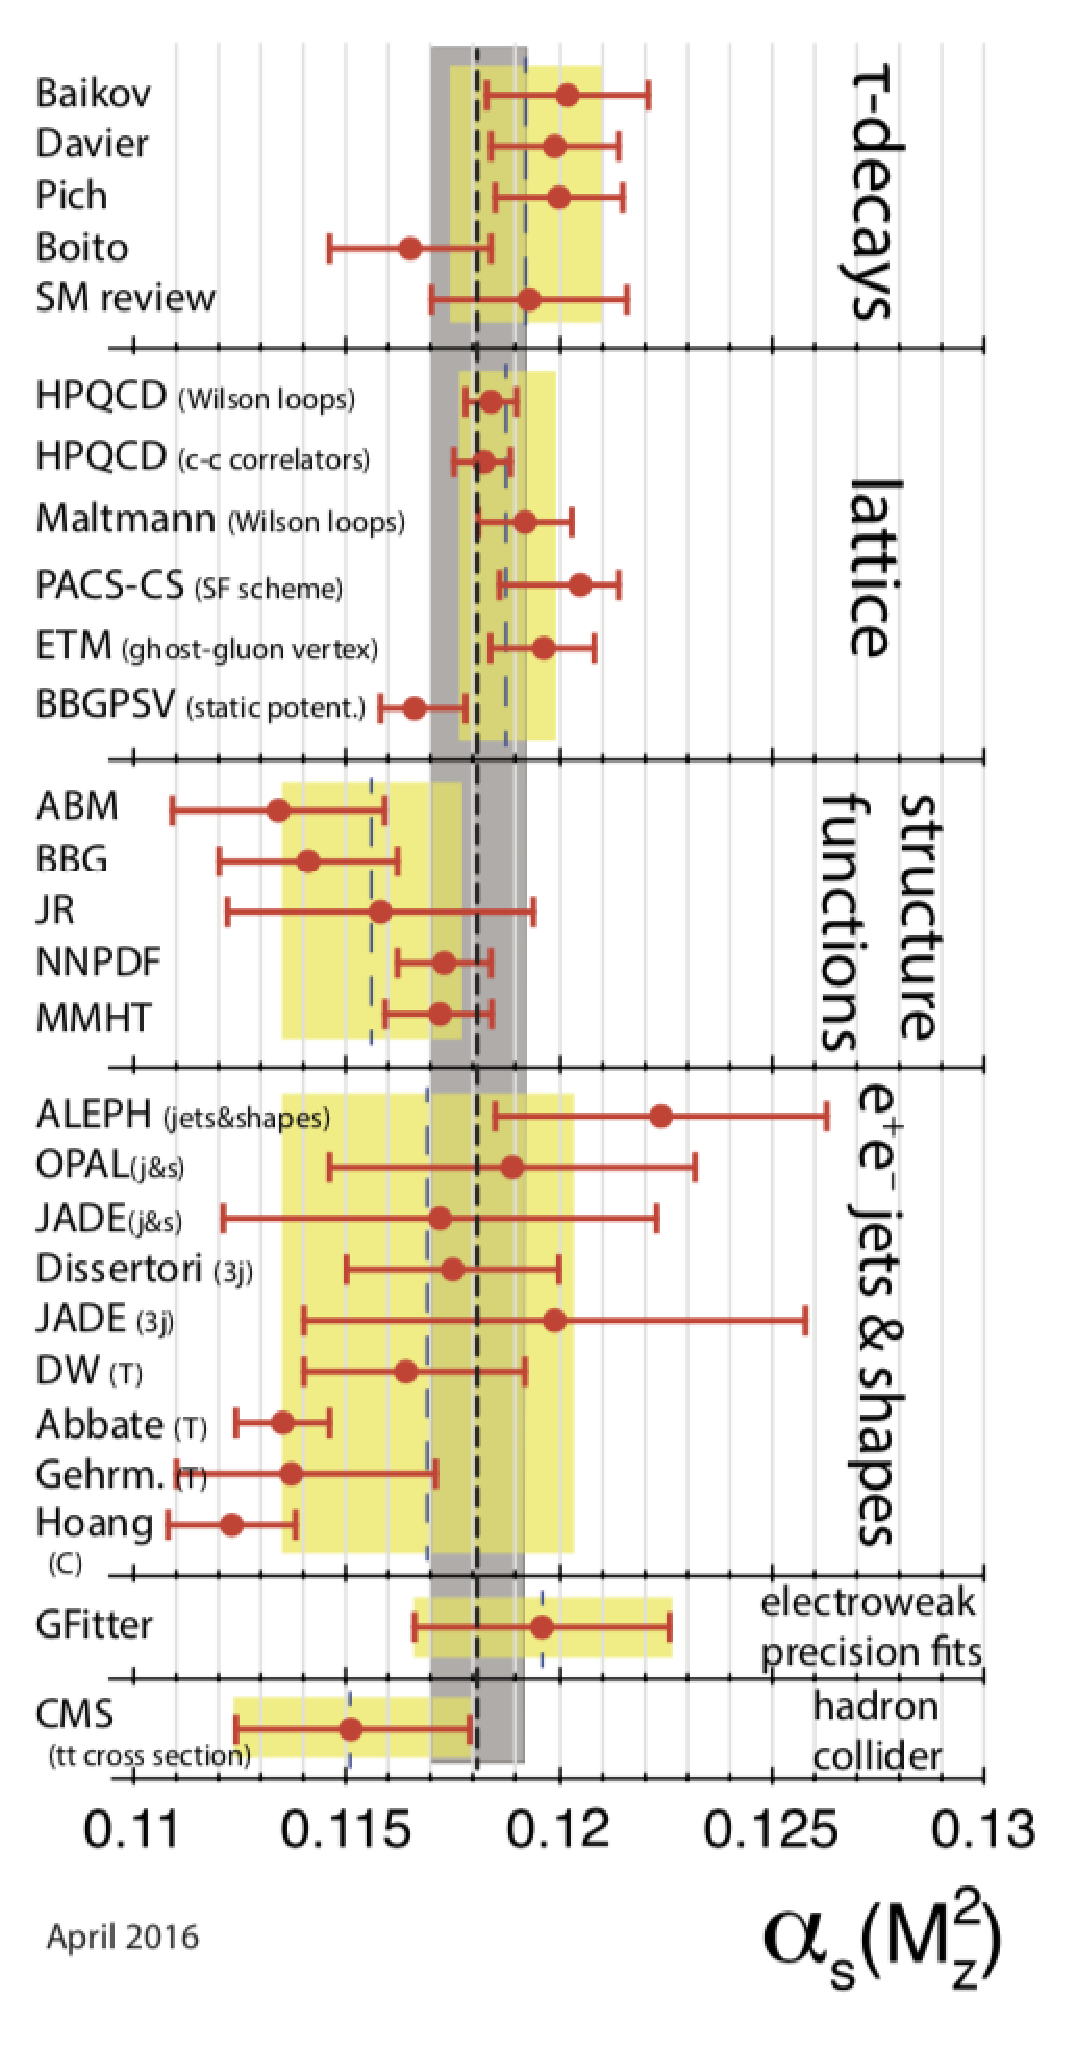
\includegraphics[width=0.33\textwidth]{./images/alphasDetermination.eps}
  \captionsetup{format=plain}
  \caption{The six different subfields and their results for measuring the
    strong coupling \(\alpha_s\) \cite{PDG2018}.}
  \label{fig:alphaSDetermination}
\end{wrapfigure}
The strong coupling is currently measured in six different ways: through
\(\tau\) decays, \textsc{qcd}\-/lattice computations, deep inelastic collider
results and electroweak precision fits \cite{PDG2018}. We have plotted the
values of each of the methods in \cref{fig:alphaSDetermination}. During this
work we will focus on the subfield of \(\tau\) decays to measure the value of
the strong coupling \(\alpha_s(m_\tau^2)\) at the \(\tau\) scale. We will see
that in \textsc{qcd} the value of the coupling ``constant'' depends upon the
scale. The \(\tau\) is an elementary particle with negative electric charge and
a spin of 1/2. Together with the lighter electron and muon it forms the group of
charged leptons\footnote{Leptons do not interact via the strong force.}. Even
though it is an elementary particle it decays via the weak interaction with a
lifetime of \(\tau_\tau=\SI{2.9e-13}{\second}\) and has a mass of
\(\SI{1776.86\pm0.12}{\mega\electronvolt}\)\cite{PDG2018}. It is furthermore the
only lepton massive enough to decay into hadrons, thus of interest for our
\textsc{qcd} analysis. The final states of a decay are limited by conservation
laws. In case of a \(\tau\) decay they must conserve the electric charge
(\(q_e=-1\)) and invariant mass of the system. Thus, we can see from the
corresponding Feynman diagram \cref{fig:tauDecay} \footnote{The \(\tau\)
  particle can also decay into strange quarks or charm quarks, but these decays
  are rather uncommon due to the heavy masses of s and c.}, that the \(\tau\)
decays by the emission of a \(W\) boson and a tau-neutrino \(\nu_\tau\) into
pairs of \((e^-, \bar\nu_e), (\mu^-, \bar\nu_\mu)\) or \((q, \bar q)\).
\begin{figure}
  \centering 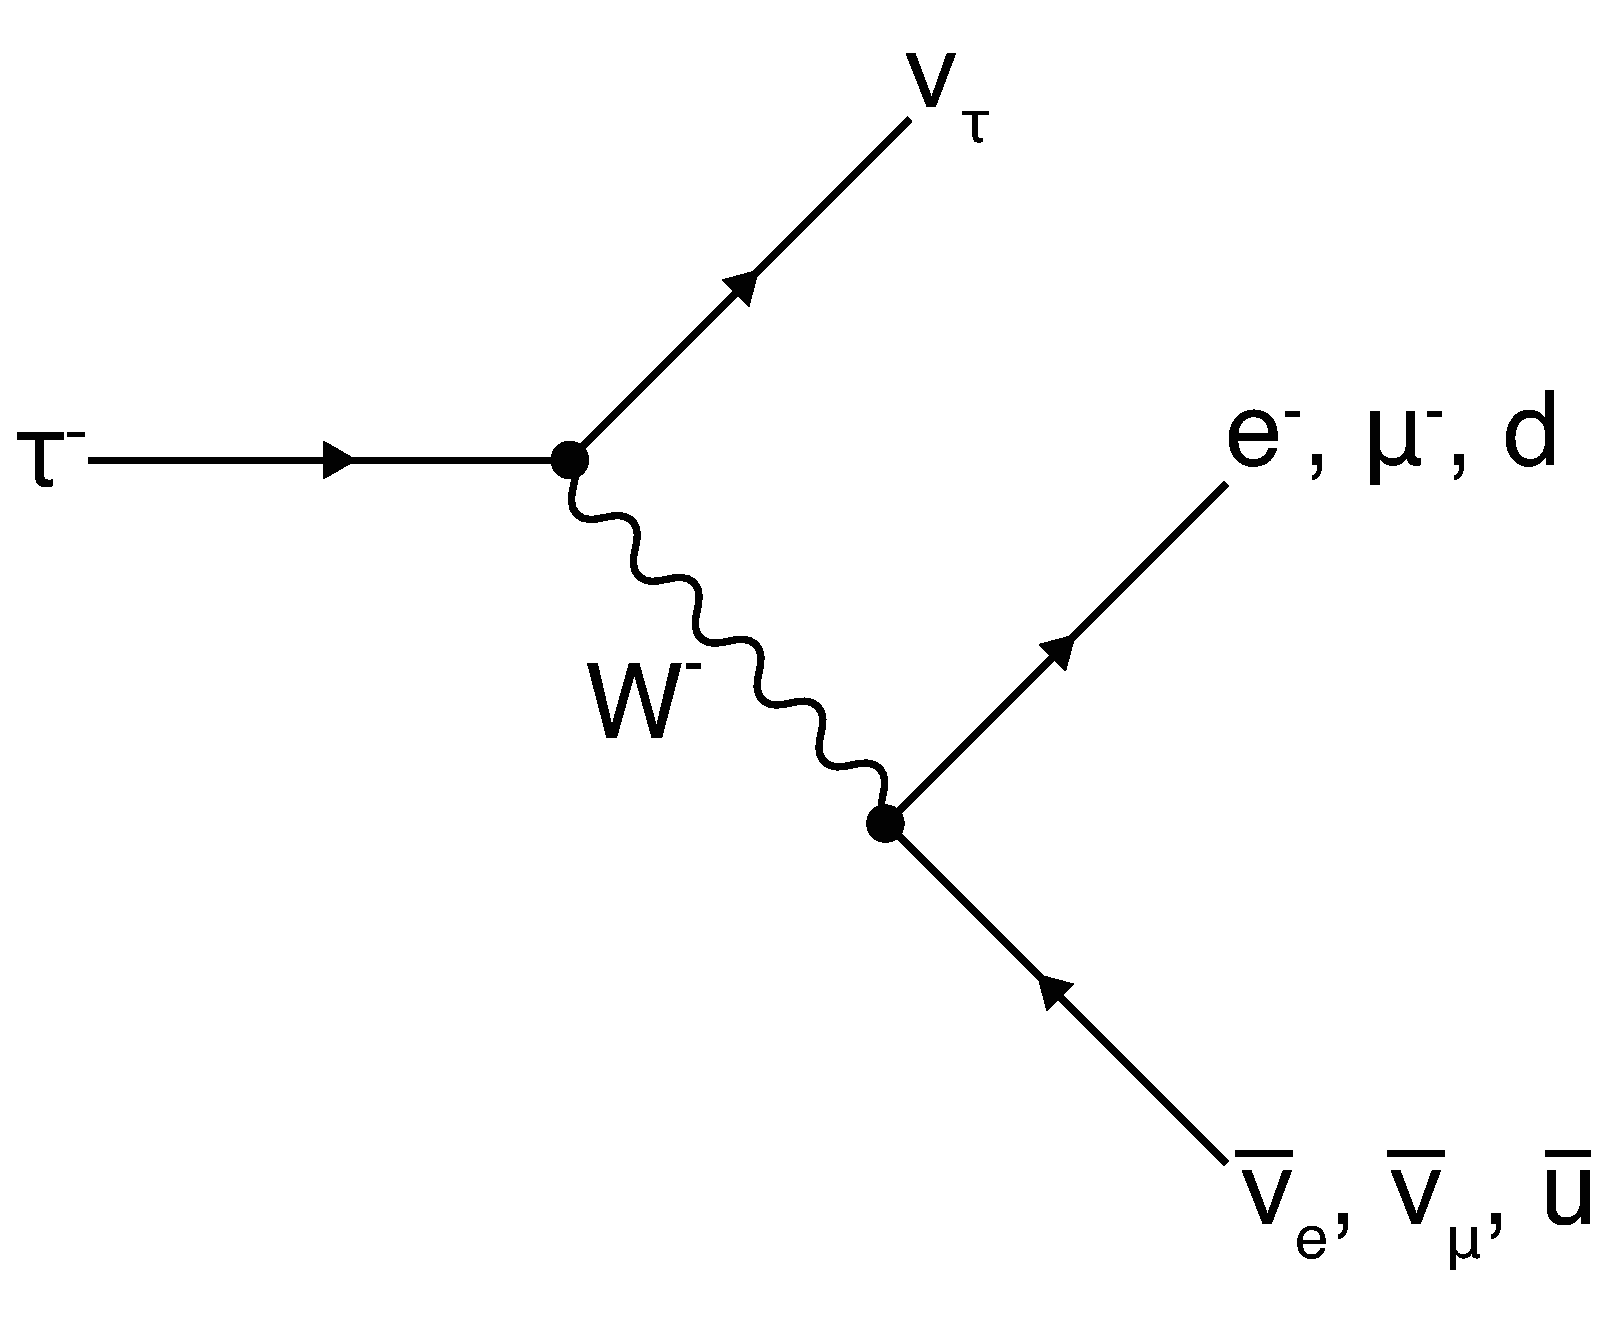
\includegraphics[width=0.4\textwidth]{images/tauDecay.eps}
  \caption{Feynman diagram of common decay of a \(\tau\)-lepton into pairs of
    lepton-antineutrino or quark-antiquark by the emission of a \textit{W
      boson}.}
  \label{fig:tauDecay}
\end{figure}
We are foremost interested into the hadronic decay channels, meaning \(\tau\)
decays that have quarks in their final states. Quarks have never been measured
isolated. Due to its mass of \(m_\tau \approx \SI{1.8}{\giga\electronvolt}\) the
\(\tau\)-particle decays into light mesons (pions (\(\pi\)), kaons (\(K\)), and
eta (\(\eta\)), see \cref{table:lightMesons}), which can be experimentally
detected.
\begin{table}
  \centering
  \begin{tabular}{lccc}
    \toprule
    Name & Symbol & Quark content & Rest mass (\(\SI{}{\mega\electronvolt}\)) \\
    \midrule
    Pion & \(\pi^-\) & \(\bar u d\) & \SI{139.57061 \pm 0.00024}{\mega\electronvolt}  \\
    Pion & \(\pi^0\) & \((u \bar u - d \bar d)/\sqrt{2}\) & \SI{134.9770\pm0.0005}{\mega\electronvolt} \\
    Kaon & \(K^-\) & \(\bar u s\) & \SI{493.677\pm0.016}{\mega\electronvolt} \\
    Kaon & \(K^0\) & \(d \bar s\) & \SI{497.611\pm0.013}{\mega\electronvolt} \\
    Eta & \(\eta\) & \((u \bar u + d \bar d - 2 s \bar s)/\sqrt{6}\) & \SI{547.862\pm0.017}{\mega\electronvolt} \\
  \end{tabular}
  \caption{List of mesons produced by a \(\tau\) decay. Rare final states with
    branching Ratios smaller than 0.1 have been omitted. The list is taken from
    \cite{Davier2006} with corresponding rest masses taken from \cite{PDG2018}.}
  \label{table:lightMesons}
\end{table}
The hadronic \(\tau\) decay provides one of the most precise ways to determine
the strong coupling \cite{Pich2016} and is theoretically accessible to high
precision within the framework of \textsc{qcd}.

The theory describing strong interactions is \textsc{qcd}. As the name
suggest\footnote{Chromo is the Greek word for colour.} \textsc{qcd} is
characterised by the colour charge and is a non-abelian gauge theory with
symmetry group \(SU(3)\). Consequently every quark has next to its type one of
the three colours blue, red or green. The colour force is mediated through eight
gluons, which each being bi\-/coloured\footnote{Each gluon carries a colour and
  an anti\-/colour.}, interact with quarks and each other. The strength of the
strong force is given by the coupling constant \(\alpha_s\), which depends on
the renormalisation scale \(\mu\). We often choose the renormalisation scale in
a way that the coupling constant \(\alpha_s(q^2)\) depends on the energy
\(q^2\). Thus the coupling varies with energy. It increases for low and
decreases for high energies\footnote{In contrast to the electromagnetic force,
  where \(\alpha(q^2)\) decreases!}. This behaviour has two main implications.
The first one states, that for low energies the coupling is too strong for
isolated quarks to exist. Until now we have not been able to observe an isolated
quark and all experiments can only measure quark compositions. These bound
states are called \textit{hadrons} and consist of two or three quarks
\footnote{There exist also so\-/called \textit{exotic hadrons}, which have more
  than three valence quarks.}, which are referred to as
mesons\footnote{Composite of a quark and an anti\-/quark.} or baryons
\footnote{Composite of three quarks or three anti\-/quarks.} respectively. This
phenomenon, of quarks sticking together as hadrons is referred to as
\textit{confinement}. As the fundamental degrees of freedom of \textsc{qcd} are
given by quarks and gluons, but the observed particles are hadrons we need to
introduce the assumption of \textit{quark\-/hadron duality} to match the theory
to the experiment. This means that a physical quantity should be similarly
describable in the hadronic picture or quark\-/gluon picture and that both
descriptions are equivalent. Quark\-/hadron duality is in general violated.
These so\-/called \define{dv}{duality violations} have an impact on our strong
coupling determinations and can be dealt with either suppression or the
inclusion of a model \cite{Cata2008}. Throughout this work we will favour and
argument for the former approach. The second implication concerns
\define{pt}{Perturbative Theory}. The lower the energies we deal with, the
higher the value of the strong coupling and the contributions of
\define{npt}{non\-/Perturbative Theory} effects. Currently there are three
solutions to deal with \define{np}{non\-/perturbative} effects:
\begin{itemize}
\item \textbf{\textit{Chiral Perturbation Theory}}
  (\textsc{chpt}\nomenclature{\textsc{chpt}}{Chiral Perturbation Theory}):
  Introduced by Weinberg \cite{Weinberg1978} in the late seventies.
  \textsc{chpt} is an effective field theory constructed with a Lagrangian
  symmetric under a chiral transformation in the limit of massless quarks. It's
  limitations are based in the chiral symmetry, which is only a good
  approximation for the light quarks \(u\), \(d\) and in some cases \(s\).
\item \textbf{\textit{Lattice QCD}}
  (\textsc{lqcd}\nomenclature{\textsc{lqcd}}{Lattice Quantum Chromodynamics}):
  Is the numerical approach to the strong force. Based on the Wilson Loops
  \cite{Wilson1974} we treat \textsc{qcd} on a finite lattice instead of working
  with continuous fields. \textsc{lqcd} has already many applications but is
  limited due to its computational expensive calculations.
\item \textbf{\textit{QCD Sum Rules}}
  (\textsc{qcdsr}\nomenclature{\textsc{qcdsr}}{Quantum Chromodynamics Sum
    Rules}): Was also introduced in the late seventies by Shifman, Vainstein and
  Zakharov \cite{Shifman1978,Shifman1978a}. It relates the observed hadronic
  picture to quark\-/gluon parameters through a dispersion relation and the use
  of the \define{ope}{operator product expansion}, which treats \textsc{np}
  effect through the definition of vacuum expectation values, the so\-/called
  \textsc{qcd} \textit{condensates}. It is a precise method for extracting the
  strong coupling \(\alpha_s\) at low energies, although limited to the unknown
  higher order contributions of the \textsc{ope}.
\end{itemize}


In this work we focus on the determination of the strong coupling \(\alpha_s\)
within the framework of \textsc{qcdsr} for \(\tau\) decays which has been
exploited in the beginning of the nineties by Braaten, Narison and Pich
\cite{Braaten1991}. Within this setup we can measure \(\alpha_s(m_\tau^2)\) at
the \(m_\tau^2\) scale. As the strong coupling gets smaller at higher energies,
so do the errors. Thus if we obtain the strong coupling at a low scale we will
obtain high precision values at the scale of the \(Z\) boson mass \(m_Z\), which
is the standard scale to compare \(\alpha_s\) values.

The \textsc{qcdsr} for the determination of \(\alpha_s\), from low energies,
contain three major issues.
\begin{enumerate}
\item There are two different approaches to treat perturbative and
  non\-/perturbative contributions. In particular, there is a significant
  difference between results obtained using \define{fopt}{fixed\-/order
    perturbation theory} or \define{cipt}{contour improved perturbation theory},
  such that analyses based on \textsc{cipt} generally arrive at about \(7\%\)
  larger values of \(\alpha_s(m_{\tau^2})\) than those based on \textsc{fopt}
  \cite{PDG2018}. There have been a variety of analyses on the topic been
  performed \cite{Pich2013,Caprini2009,Jamin2005} and we will favour the
  \textsc{fopt} approach, but generously list our results for the \textsc{cipt}
  framework.

\item There are several prescriptions to deal with the \textsc{np} contributions
  of higher order \textsc{ope} condensates. Typically terms of higher dimension
  have been neglected, even if they knowingly contribute. In this work we will
  include every necessary \textsc{ope} term.

\item Finally there are known \textsc{dv} leading to an ongoing discussion of
  the importance of contributions from \textsc{dv}. Currently there are two main
  approaches: Either we neglect them, arguing that they are sufficiently
  suppressed due to \textit{pinched weights} \cite{Pich2016} or model
  \textsc{dv} with sinusoidal exponentially suppressed function
  \cite{Cata2008,Boito2011a,Boito2014} introducing extra fitting parameters. We
  will argue for the former method, implementing pinched weights that
  sufficiently suppress \textsc{dv} contributions such as having only a
  negligible effect on our analysis.
\end{enumerate}

In the following chapter of this work we want to summarise the necessary theoretical
background for working with the \textsc{qcdsr}. Starting with the basics of
\textsc{qcd} we want to motivate the \define{rge}{Renormalisation Group
  Equation}, which is responsible for the running of the strong coupling. We
then continue with the two\-/point function and its usage in the dispersion
relation, which connects the hadronic picture with the quark\-/gluon picture.
Then we introduce the \textsc{ope} to treat the \textsc{np} part of
\textsc{qcd}, before we combine everything to formulate \textsc{qcdsr}. In the
third chapter we will apply the abstract theory gathered in the second chapter
to \(\tau\) decays. In the fourth chapter we will state and interpret our fitting
results before concluding in the last chapter.


\end{document}
% LocalWords:  SMTaxonomy tauDecay alphaSDetermination lightMesons lccc
